\documentclass[landscape, 8pt]{extarticle}
\usepackage{geometry}
% \usepackage{showframe}
\usepackage[dvipsnames]{xcolor}

\colorlet{colour1}{Red}
\colorlet{colour2}{Green}
\colorlet{colour3}{Cerulean}

\geometry{
	a4paper, 
	margin=0.17in
}

\pretolerance=0
\hyphenpenalty=0

\usepackage{lmodern}

\usepackage[fontsize=7pt]{scrextend}

\usepackage{pgfplots}
\pgfplotsset{width=200pt,compat=1.9}


\usepackage{graphicx} % Required for inserting images
\usepackage{amsmath}
\usepackage{amsfonts}
\usepackage{amssymb}
% \usepackage{preamble}
\usepackage{enumitem}
\usepackage{multicol}
\usepackage{lipsum}
\usepackage[framemethod=TikZ]{mdframed}
% \usepackage{../thmboxes_white}
\usepackage{../thmboxes_v2}
\usepackage{float}
% \usepackage{setspace}
\usepackage[nodisplayskipstretch]{setspace}





% \setlength{\parskip}{0pt}

% Custom Definitions of operators
% \DeclareMathOperator{\im}{im}
% \DeclareMathOperator{\Fix}{Fix}
% \DeclareMathOperator{\Orb}{Orb}
% \DeclareMathOperator{\Stab}{Stab}
% \DeclareMathOperator{\send}{send}
\DeclareMathOperator{\dom}{dom}
% \DeclareMathOperator{\Maps}{Maps}
% \DeclareMathOperator{\sgn}{sgn}
% \DeclareMathOperator{\Mat}{Mat}
% \DeclareMathOperator{\scale}{sc}
% \DeclareMathOperator{\Hom}{Hom}
% \DeclareMathOperator{\id}{id}
% \DeclareMathOperator{\rk}{rk}
% \DeclareMathOperator{\Tr}{tr}
% \DeclareMathOperator{\diag}{diag}
% \DeclareMathOperator{\can}{can}

\usepackage{hyperref} % note: this is the final package

\parindent = 0pt

\renewcommand\labelitemi{\tiny$\bullet$}

\begin{document}

\setlength{\abovedisplayskip}{3.5pt}
\setlength{\belowdisplayskip}{3.5pt}
\setlength{\abovedisplayshortskip}{3.5pt}
\setlength{\belowdisplayshortskip}{3.5pt}

\begin{multicols}{3}
\raggedcolumns


\section*{\huge Honours Analysis Exam Notes}
Made by Leon :) \textit{Note: Any reference numbers are to the lecture notes}

\vspace{-5pt}
\section{Revisiting FPM}

\begin{dfn}[Nested Sequences and covers]{dfn:nested-sequence}{1.1}
	A sequence $(I_{n})_{n\in\mathbb{N}}$ of sets is said to be \textbf{nested} if
	\[I_{1} \subset I_{2} \subset I_{3} \subset \cdots\]

	\noindent\rule{\textwidth}{0.2pt}
	\textbf{Thm 1.1}: If $(I_{n})$ is a nested sequence of nonempty closed bounded intervals then
	$$E = \bigcap\limits_{n\in\mathbb{N}} I_{n} = \{x\in\mathbb{R}: x\in I_{n},\,\forall n\in\mathbb{N}\}$$
	is nonempty (i.e. it contains at least one number). Moreover if $\lambda(I_{n})\to 0$, where $\lambda(I_{n})$ denotes the length of interval $I_{n}$, then $E$ contains exactly one number

	\noindent\rule{\textwidth}{0.2pt}
	\textbf{Thm 1.2}: Let $E$ be a subset of $\mathbb{R}^n$
	\begin{itemize}
		\setlength\itemsep{0em}
		\item A \textbf{cover} of $E$ is a collection of sets  $\{I_{\alpha}\}_{\alpha\in A}$ such that
			\[E\subseteq \bigcup\limits_{\alpha\in A} I_{\alpha}\]
		\item An \textbf{open covering} of $E$ is a cover such that each $I_{\alpha}$ is open, i.e.$(a,b)$ compared to $[a,b]$
		\item A \textbf{finite subcover} of $E$ is a collection of sets $(I_{\alpha})_{\alpha\in A_{0}}$ where there exists a subset $A_{0} = \{\alpha_{1}, \alpha_{2}, \dots, a_{N}\}$ of $A$ such that $(I_{\alpha})_{\alpha\in A_{0}}$ is a finite subset of $(I_{\alpha})_{\alpha\in A}$ that is also a cover
		\item The set $E$ is said to be \textbf{compact} iff every open covering of $E$ has a \textbf{finite subcovering}; that is
			\[E\subseteq \bigcup\limits_{j=1}^{N} I_{aj} \quad \text{ or } \quad E \subseteq I_{\alpha_{1}} \cup I_{a_{2}} \cup \cdots \cup I_{a_{N}}\]
	\end{itemize}
\end{dfn}

\begin{dfn}[Convergence of Sequences and Cauchy]{dfn:epsilon-n-sequences}{1.2}

	A sequence of real numbers $(x_{n})$ is said to \textbf{converge} to a real number $a\in \mathbb{R}$ iff for every $\epsilon>0$ there is an $N\in\mathbb{N}$ such that

	\vspace{-5pt}
	\[n\ge N \text{ implies } \lvert x_{n} - a \rvert < \epsilon\]
	If $(x_{n})$ converges to $a$, we will write $\lim_{n \to \infty} x_{n}=a$, or $x_{n}\to a$. The number $a$ is called the limit of the sequence $(x_{n})$. A sequence that does not converge to some real number is said to *diverge

	\noindent\rule{\textwidth}{0.2pt}
	\textbf{Def 1.3}: A sequence $(x_{n})$ of numbers $x_{n} \in \mathbb{R}$ is said to be \textbf{Cauchy} if for every $\epsilon > 0$ there is $N\in \mathbb{N}$ such that
	\[\lvert x_{n} - x_{m} \rvert < \epsilon \quad \forall n,m\ge N\]

\end{dfn}

\begin{dfn}[Subsequences]{dfn:subsequence}{1.4}
	Suppose $(x_{n})_{n\in\mathbb{N}}$ is a sequence. A subsequence of this sequence is a sequence of the form $(x_{n_{k}})_{k\in\mathbb{N}}$ where for each $k$ there is a positive integer $n_{k}$ such that

	\vspace{-5pt}
	\[n_{1} < n_{2} < \cdots < n_{k} < n_{k+1} < \cdots\]
	Thus, $(x_{n})_{n\in\mathbb{N}}$ is just a selection of some (possibly all) of the $x_{n}$'s taken in order

\end{dfn}


\begin{dfn}[Limit Superior and Inferior]{dfn:limsup-liminf}{1.5}
	If $(x_{n})$ is a bounded sequence of real numbers we denote by

	\vspace{-5pt}
	\[\limsup_{{n\to\infty}} x_{n} = \lim_{n \to \infty} \left(\displaystyle \sup_{k\ge n} x_{k}\right),\,\qquad \liminf_{{n\to\infty}} x_{n} = \lim_{n \to \infty} \left(\displaystyle \inf_{k\ge n} x_{k}\right)\]

	\noindent\rule{\textwidth}{0.2pt}
	\textbf{Note}: These are only defined for bounded sequences

	\vspace{-5pt}
	\begin{itemize}[leftmargin=*]
		\setlength\itemsep{0em}
		\item If $(x_{n})$ is not bounded above then we write $\limsup_{n \to \infty} x_{n} = +\infty$

		\item If $(x_{n})$ is not bounded below then we write $\liminf_{n \to \infty} x_{n} = +\infty$
	\end{itemize}
	\vspace{-5pt}
\end{dfn}

\vspace{-5pt}
\begin{dfn}[Continuity]{dfn:continuity}{1.7}
	\vspace{-5pt}
	Define $f : \dom(f) \to \mathbb{R}$ where $\dom(f)\subset \mathbb{R}$. $f$ is \textbf{continuous} at some $a\in \dom(f)$, if for any sequence $(x_{n})$ whose terms lie in $\dom(f)$ and converges to $a$, we have $\lim_{n\to \infty} f(x_{n}) = f(a)$.

	% If $f$ is continuous at each $a\in S \subset \dom(f)$ then we say $f$ is continuous on $S$. If $f$ is continuous of $\dom(f)$ then we say $f$ is continuous

	\noindent\rule{\textwidth}{0.2pt}
	\textbf{Thm 1.10}: Let $f, g : D \to \mathbb{R}$ be continuous on $D$, and let $\alpha\in \mathbb{R}$. Then the following functions are continuous on $D:$

	\vspace{-10pt}
	\begin{multicols}{3}
		\begin{enumerate}
			\item $\alpha$ f
			\item $f + g$
			\item $fg$
		\end{enumerate}
	\end{multicols}

	\vspace{-5pt}
	\vspace{-10pt}
	\noindent\rule{\textwidth}{0.2pt}

	\textbf{Thm 1.12 ($\epsilon-\delta$ Definition of Continuity)}: A function $f : A \to \mathbb{R}$ is \textbf{continuous} at $x$ iff for any $\epsilon > 0$ there exists $\delta > 0$ s.t.
	\[\lvert x - a \rvert < \delta\text{ implies }\lvert f(x) - f(a) \rvert < \epsilon\]

	\textbf{Thm (Uniform Continuity)}: A function $f : A \to \mathbb{R}$ is \textbf{uniformly continuous} at $x$ iff for any $\epsilon > 0$ there exists $\delta > 0$ s.t. $\forall x,y\in A$,
	\[\lvert x - y \rvert < \delta\text{ implies }\lvert f(x) - f(y) \rvert < \epsilon \]

	\textbf{Thm (Inverse)}: A function $f : A \to \mathbb{R}$ is \textbf{not} continuous if for all $\delta>0$ there exists $\epsilon > 0$ s.t. there exists some $x,a\in A$ where
	\[\lvert x - a \rvert < \delta \text{ but } \lvert f(x) - f(a) \rvert \ge \epsilon\]

	\vspace{-5pt}
	\noindent\rule{\textwidth}{0.2pt}

	\textbf{Thm 1.13 (Intermediate Value Theorem)}: Let $a < b$ real numbers and $f : [a, b] \to \mathbb{R}$ be continuous on $[a, b]$. If $f(a)f(b)<0$ then there exists at least one $c\in (a, b)$ s.t. $f(c) = 0$

	\noindent\rule{\textwidth}{0.2pt}

	\textbf{Thm 1.14 (Extreme Value Theorem)}: Let $a < b$ real numbers and $f : [a, b]\to \mathbb{R}$ be continuous on $[a, b]$. Then there exists points $c, d\in [a,b]$ s.t.
	\[f(c) = \inf \{f(x) : x\in [a, b]\}, \quad f(d) = \sup \{f(x) : x\in [a, b]\}\]
	That is, the function $f$ on the interval $[a, b]$ is bounded and attains its minimal value at some point $c\in [a,b]$. Similarly, the maximal value of $f$ is also attained at some point $d\in [a,b]$
\end{dfn}

\vspace{-7pt}
\begin{dfn}[Convergent Infinite Series]{dfn:convergent-infinite-series}{1.6}
	\vspace{-5pt}
	Let $S=\sum_{k=1}^{\infty}a_{k}$ be an infinite series $a_{k}$. For each $n\in\mathbb{N}$, the partial sum of $S$ of order $n$ is defined by

	\vspace{-8pt}
	\[s_{n} = \sum_{k=1}^{n} a_{k}\]

	\vspace{-5pt}
	$S$ is said to \textbf{converge} iff its sequence of partial sums $(s_{n})$ converges to some $s \in\mathbb{R}$ as $n\to\infty$; that is, iff for every $\epsilon>0$ there is an $N\in\mathbb{N}$ s.t. for all $n\ge N$ we have $\lvert s_{n}-s \rvert < \epsilon$. In this case we shall write

	\vspace{-7pt}
	\[\sum_{k=1}^{\infty} a_{k} = s\]
	\vspace{-3pt}
	and call $s$ the \textbf{sum} or \textbf{value} of the series $\sum_{k=1}^{\infty}a_{k}$

	\noindent\rule{\textwidth}{0.2pt}

	\vspace{-5pt}
	\begin{itemize}[leftmargin=*]
	    \setlength\itemsep{0em}
	    \item \textbf{Absolutely convergent}: the series $\sum_{k = 1}^{\infty} \lvert a_{k} \rvert$ is convergent
	    \item \textbf{Conditionally convergent}: Convergent but not absolutely
	\end{itemize}
\end{dfn}


% idk where i got this guy actually?

% \begin{thm}[Cauchy Criteron]{thm:cauchy-criteron}{1.7}
% 	Let $\{a_{k}\}$ be a real sequence. Then the infinite series $\sum_{k=1}^{\infty} a_{k}$ converges if and only if given $\epsilon>0$ there is an $N\in\mathbb{N}$ such that
%
% 	\[n\ge N \text{ implies } \left\lvert  \sum_{k=n}^{\infty} a_{k}  \right\rvert <\epsilon\]
% \end{thm}

\vspace{-5pt}
\begin{dfn}[Composition]{dfn:composition}{1.8}
	Let $A, B \subseteq \mathbb{R}$ be nonempty, let $f : A \to \mathbb{R},\, g : B \to \mathbb{R}$ and $f(A) \subseteq B$. The composition of $g$ with $f$ is the function $g \circ f : A \to \mathbb{R}$ defined by
	\[(g \circ f)(x) = g(f(x)), \quad \text{for all $x\in A$}\]

	\vspace{-5pt}
	\noindent\rule{\textwidth}{0.2pt}

	\textbf{Thm 1.11}: If $f$ is continuous at $a\in \mathbb{R}$ and $g$ is continuous at $f(a)$ then the composition $g \circ f$ is continuous at $a$
\end{dfn}

\vspace{-15pt}
\section{Uniform convergence}

\begin{dfn}[Pointwise Convergence]{dfn:pointwise-convergence}{2.1}
	\vspace{-5pt}
	Let $E \subset \mathbb{R}$, $E$ nonempty. A sequence of functions $f_{n}: E\to \mathbb{R}$ is said to \textbf{converge pointwise} on $E$, written $f_{n}\to f$ pointwise on $E$ as $n\to \infty$, iff $f(x) = \lim_{n \to \infty}f_{n}(x)$ exists for each $x \in E$

	\noindent\rule{\textwidth}{0.2pt}
	$f_{n}$ \textbf{converges pointwise} on $E$, as $n\to\infty$, iff for every $\epsilon>0$ and $x \in E$ there's an $N \in\mathbb{N}$ (which may depend on $x$ as well as $\epsilon$) s.t.

	\vspace{-8pt}
	\[n\ge N\quad\text{implies}\quad \lvert f_{n}(x)-f(x) \rvert < \epsilon\]

	\vspace{-5pt}
	\noindent\rule{\textwidth}{0.2pt}
	\textbf{Remarks}:
	\vspace{-5pt}
	\begin{itemize}[leftmargin=*]
		\setlength\itemsep{0em}
		\item The pointwise limit of continuous (or differentiable) functions is not necessarily continuous (or differentiable).

		\item The pointwise limit of integrable functions is not always integrable.

		\item There exist continuous functions $f_{n}$ and $f$ such that $f_{n}\to f$ pointwise on $[0,1]$ but

			\vspace{-5pt}
			\[\lim_{n \to \infty} \int_{0}^{1} f_{n}(x) \, dx \ne \int_{0}^{1} \left(\lim_{n \to \infty} f_{n}(x)\right) \, dx \]
	\end{itemize}

	\noindent\rule{\textwidth}{0.6pt}

	\textbf{Def 2.2}: Let $E$ be a nonempty subset of $\mathbb{R}$. A sequence of functions $f_{n}: E\to\mathbb{R}$ is said to \textbf{converge uniformly} on $E$ to a function $f$ (notation: $f_{n}\to f$ uniformly on $E$ as $n\to\infty$) if and only if for every $\epsilon>0$ there is an $N \in\mathbb{N}$ such that for all $x \in E$

	\vspace{-8pt}
	\[n\ge N\quad\text{implies}\quad \lvert f_{n}(x)-f(x) \rvert <\epsilon\]

	\vspace{-5pt}
	\noindent\rule{\textwidth}{0.2pt}
	\textbf{Remark (The difference between Pointwise and Uniform)}: For a sequence of functions to be pointwise convergent, it is enough to have an $N_{n}$ for every $x_{n}$, but for it to be uniformly convergent, it has to have \textbf{the same} $N$ for every $x$ in the sequence

	\noindent\rule{\textwidth}{0.2pt}

	\textbf{Def 2.2}: A sequence of functions $f_{n}$ is said to be \textbf{uniformly bounded} on a set $E$ if there is a $M>0$ such that $\lvert f_{n}(x) \rvert\le M$ for all $x\in E$ and all $n\in N$
\end{dfn}

\vspace{-5pt}
\begin{dfn}[Convergence of series]{dfn:convergence-of-sequence}{2.3}
	\vspace{-5pt}
	Let $f_{k}$ be a sequence of real functions defined on some set $E$ and set

	\vspace{-5pt}
	\[s_{n}(x)=\sum_{k=1}^{n} f_{k}(x),\quad x\in E,\,n\in \mathbb{N}\]
	\begin{itemize}
		\setlength\itemsep{0em}
		\item The series $\sum_{k=1}^{\infty} f_{k}$ \textbf{converges pointwise} on $E$ iff the sequence $s_{n}(x)$ converges pointwise on $E$ as $n\to\infty$

		\item The series $\sum_{k=1}^{\infty} f_{k}$ \textbf{converges uniformly} on $E$ iff the sequence $s_{n}(x)$ converges uniformly on $E$ as $n\to\infty$

		\item The series $\sum_{k=1}^{\infty} f_{k}$ \textbf{converges absolutely} (pointwise) on $E$ iff $\sum_{k=1}^{\infty} \lvert f_{k}(x) \rvert$ converges for each $x\in E$

	\end{itemize}
\end{dfn}

\newpage
\begin{dfn}[All about Power Series]{dfn:power-series}{3.1}
	\vspace{-5pt}
	The \textbf{radius of convergence} $R$ of the power series

	\vspace{-8pt}
	\begin{equation}
		\sum_{n=0}^{\infty} a_{n}(x-c)^{n}\tag{$*$}\label{$*$}
	\end{equation}
	is defined by $R=\sup\{r\ge 0:(a_{n}r^n) \text{ is bounded}\}$, unless $(a_{n}r^{n})$ is bounded for all $r\ge 0$, where we say that $R=\infty$

	\noindent\rule{\textwidth}{0.2pt}

	\textbf{Thm 3.1}: Suppose the radius of convergence $R$ of \ref{$*$} satisfies $0<R<\infty$. If $\lvert x-c \rvert<R$, the power series \ref{$*$} converges absolutely. If $\lvert x-c \rvert>R$, the power series \ref{$*$} diverges

	\vspace{-5pt}
	\noindent\rule{\textwidth}{0.2pt}

	\textbf{Thm 3.2 (Continuity of Power Series)}: Assume that $R>0$. Suppose that $0<r<R$. Then a power series converges uniformly and absolutely on $\lvert x-c \rvert\le r$ to a continuous function $f$. Hence

	\vspace{-8pt}
	\[f(x)=\sum_{n=0}^{\infty} a_{n}(x-c)^{n}\]
	defines a continuous function $f:(c-R,c+R)\to \mathbb{R}$

	\vspace{-5pt}
	\noindent\rule{\textwidth}{0.2pt}
	\textbf{Lemma 3.1}: The two power series

	\vspace{-8pt}
	\[\sum_{n=1}^{\infty} a_{n}(x-c)^{n}\text{ and } \sum_{n=1}^{\infty} na_{n}(x-c)^{n-1}\]
	have the same radius of convergence

	\vspace{-5pt}
	\noindent\rule{\textwidth}{0.2pt}
	\textbf{Thm 3.3 (Differentiation of Power Series)}: Suppose the radius of convergence of a power series is $R$. Then the function

	\vspace{-8pt}
	\[f(x)=\sum_{n=0}^{\infty} a_{n}(x-c)^{n}\]
	is infinitely differentiable on $\lvert x-c \rvert<R$, and for such $x$,
	\vspace{-8pt}

	\[f'(x)=\sum_{n=0}^{\infty} na_{n}(x-c)^{n-1}\]
	and the series converges absolutely, and also uniformly on $[c-r,c+r]$ for any $r<R$. Moreover,

	\vspace{-5pt}
	\[a_{n}=\frac{f^{(n)}(c)}{n!}\]
\end{dfn}

% TODO: maybe some stuff on exponential function (pg 32)


\vspace{-15pt}
\section{Lebesgue Integration}

\vspace{-5pt}
\begin{dfn}[Characteristic Function]{dfn:characteristic-function}{4.0}
	\vspace{-5pt}
	Let $E$ be a subset of $\mathbb{R}$. We define its \textbf{characteristic function} $\chi_{E}:\mathbb{R}\to\mathbb{R}$ by $\chi_{E}(x)=1$ if $x\in E$ and $\chi_{E}(x)=0$ if $x\not\in E$. i.e.,
	\[\chi_{E}=\begin{cases}
	1&x\in E \\
	0 & x\not\in E
	\end{cases}\]
	i.e. it's $1$ at all points of a bounded interval, and $0$ elsewhere

	\vspace{-5pt}
	\noindent\rule{\textwidth}{0.2pt}
	
	Let $I$ be a bounded interval with endpoints $a,\,b$ and $a\le b$. We call the number $b-a$ the \textbf{length of the interval} $I$ and we denote it by $\lambda(I)$. This might also be referred to as $\lvert I \rvert$. That is,
	\[\lambda((a,b)) = \lambda([a,b]) = \lambda((a,b]) = \lambda([a,b)) = b-a\]

	\vspace{-5pt}
	\noindent\rule{\textwidth}{0.2pt}
	From our definition of a characteristic function and the length of an interval, we have that the area of the characteristic function is a rectangle with width $\lambda(I)$ and height $1$, therefore
	\vspace{-3pt}
	\[\int \chi_{I} = 1 \cdot \lambda(I) = \lambda(I)\]
\end{dfn}

\begin{dfn}[Step function]{dfn:step-function}{4.1}
	\vspace{-5pt}
	We say that $\phi:\mathbb{R}\to \mathbb{R}$ is a \textbf{step function} if there exist real numbers $x_{0}<x_{1}<x_{2}<\cdots<x_{n}$ (for some $n\in \mathbb{N}$) such that

	\vspace{-5pt}
	\begin{enumerate}
	    \setlength\itemsep{0em}
	    \item $\phi(x)=0$ for $x<x_{0}$ and $x>x_{n}$
	    \item $\phi$ is constant on $(x_{j-1}, x_{j})$ for $1\le j \le n$
	\end{enumerate}

	\vspace{-5pt}
	We shall use the phrase "$\phi$ is a step function with respect to $\{x_{0},x_{1},\dots,x_{n}\}$" to describe this situation


	\noindent\rule{\textwidth}{0.2pt}

	\textbf{Properties of Step Functions}

	\vspace{-5pt}
	\begin{enumerate}
	    \setlength\itemsep{0em}
	    \item The class of step functions is a vector space - i.e. if $\phi$ and $\psi$ are step functions and $\alpha$ and $\beta$ are real numbers, then $\alpha\phi+\beta\psi$ is a step function, and that if $\phi$ and $\psi$ are step functions, then $\max\{\phi,\psi\}$, $\min\{\phi\psi\}$, $\lvert \phi \rvert$ and $\phi\psi$ are also step functions
	    \item If $\phi$ and $\psi$ are step functions, then $\phi + \psi$ is a step function
	    \item $\phi$ is a step function if and only if it is of the form
	\[\phi=\sum_{j=1}^{n} c_{j}\chi_{J_{j}}\]
	for some $n$, $c_{j}$, and bounded intervals $J_{j}$
	\end{enumerate}

	\vspace{-8pt}
	\noindent\rule{\textwidth}{0.2pt}

	\textbf{Def 4.2: Integral of a Step Function}

	If $\phi$ is a step function with respect to $\{x_{0},x_{1},\dots,x_{n}\}$ which takes the value $c_{j}$ on $(x_{j-1},x_{j})$, then
	\[\int \phi := \sum_{j=1}^{n} c_{j}(x_{j}-x_{j-1})\]
	Therefore, using the $\chi(x)$ definition of a step function, the integral is
	\[\int \phi = \int \sum_{j=1}^{n} c_{j}\chi_{J_{j}}=\sum_{j=1}^{n} c_{j}\int \chi_{IJ_{j}}=\sum_{j=1}^{n} c_{j}\lambda(J_{j})\]
\end{dfn}

\vspace{-5pt}
\begin{dfn}[Lebesgue Integrals]{dfn:lebesgue-integral}{4.3}
	A function $f:I\to \mathbb{R}$ is said to be \textbf{integrable} or more precisely \textbf{Lebesgue integrable} on an interval $I$ if there exist numbers $c_{j}$ and bounded intervals $J_{j}\subset I,\,j=1,2,3,\dots$ such that
	\[\sum_{j=1}^{\infty} \lvert c_{j} \rvert \lambda(J_{j})<\infty\]
	and the equality
	\vspace{-5pt}
	\[f(x)=\sum_{j=1}^{\infty} c_{j}\chi_{J_{j}}(x)\]
	holds for all $x\in I$ at which
	\[\sum_{j=1}^{\infty} \lvert c_{j} \rvert \chi_{J_{j}}(x)<\infty\]
	We denote by $\int_{I}f$ the number
	\[\int _{I}f=\sum_{j=1}^{\infty} c_{j}\lambda(J_{j})\]
	and call it the \textbf{integral of $f$ over the interval $I$}.
	If the function $f$ is not integrable on the interval $I$ then we say that the integral of $f$ on $I$ does not exist. Hence if we say that the integral of $f$ on $I$ exists it just means that $f$ is (Lebesgue) integrable on $I$.
\end{dfn}

\begin{thm}[Lebesgue Equality]{thm:lebesgue-equality}{4.1}
	Suppose that $c_{j}$, $d_{j}$ are real numbers and $J_{j}$, $K_{j}$ are bounded intervals for all $j=1,2,3,\dots$, and
	\[\sum_{j=1}^{\infty} \lvert c_{j} \rvert \lambda(J_{j})<\infty,\quad \sum_{j=1}^{\infty} \lvert d_{j} \rvert \lambda(K_{j})<\infty\]
	If
	\[\sum_{j=1}^{\infty} c_{j}\chi_{J_{j}}(x)=\sum_{j=1}^{\infty} d_{j}\chi_{K_{j}}(x)\]
	holds for all $x$ such that
	\[\sum_{j=1}^{\infty} \lvert c_{j} \rvert \chi_{J_{j}}(x)<\infty,\quad \sum_{j=1}^{\infty} \lvert d_{j} \rvert \chi_{K_{j}}(x)<\infty\]
	Then
	\[\sum_{j=1}^{\infty} c_{j}\lambda(J_{j})=\sum_{j=1}^{\infty} d_{j}\lambda(K_{j})\]
\end{thm}


\begin{dfn}[Riemann Integrable Functions]{dfn:riemann-integrable}{4.4}
	\vspace{-5pt}
	Let $f : \mathbb{R} \to \mathbb{R}$. We say that $f$ is \textbf{Riemann-integrable} if for every $\epsilon > 0$ there exists step functions $\phi$ and $\psi$ such that
	\[\phi \le f \le \psi\]
	and
	\[\int \psi - \int \phi < \epsilon\]

	\noindent\rule{\textwidth}{0.2pt}
	\textbf{Thm 4.5}: A function $f : \mathbb{R}\to \mathbb{R}$ is Riemann-integrable iff
	\begin{align*}
		& \sup \left\{\int \phi : \text{$\phi$ is a step function and $\phi \le f$}\right\} \\
		= & \inf \left\{\int \psi : \text{$\psi$ is a step function and $\phi \ge f$}\right\}
	\end{align*}

	\noindent\rule{\textwidth}{0.2pt}
	\textbf{Def 4.5}: If $f$ is Riemann-integrable we define its Riemann integral $(R) \int f$ as the common value
	\begin{align*}
		(R) \int f&:= \sup \left\{\int \phi : \text{$\phi$ is a step function and $\phi \le f$}\right\} \\
		&= \inf \left\{\int \psi : \text{$\psi$ is a step function and $\phi \ge f$}\right\}
	\end{align*}
\end{dfn}

\begin{thm}[Connection between Riemann and Lebesgue]{thm:riemann-lebesgue-connection}{4.6}
	Suppose that $f : \mathbb{R} \to \mathbb{R}$ is Riemann-integrable. Then $f$ is also Lebesgue integrable on $\mathbb{R}$ and moreoever
	\[(R) \int f = \int f\]
	where the number on the lefthand side is the value of the Riemann integral of $f$, while the righthand side denotes the value of the Lebesgue integral of $f$ on $\mathbb{R}$
\end{thm}

\newpage
\vspace{-6pt}
\begin{thm}[Riemann lemmas]{thm:riemann-lemmas}{4.1}
	\vspace{-5pt}
	Let $f : \mathbb{R} \to \mathbb{R}$ be a bounded function with bounded support $[a, b]$. The following are equivalent:

	\vspace{-5pt}
	\begin{enumerate}[leftmargin=*]
	    \item $f$ is Riemann-integrable
			\vspace{-3pt}
	    \item for every $\epsilon > 0$ there exists $a = x_{0} < \cdots < x_{n} = b$ s.t. if $M_{j}$ and $m_{j}$ denote the sup and inf of $f$ on $(x_{j-1}, x_{j})$ respectively, then

			\vspace{-13pt}
			\[\sum_{j = 1}^{n}(M_{j} - m_{j})(x_{j} - x_{j - 1}) < \epsilon\]
		\item for every $\epsilon > 0$ there exists $\alpha = x_{0} < \cdots < x_{n} = b$ s.t. with $I_{j} = (x_{j-1}, x_{j})$ for $j \ge 1$
			\[\sum_{j = 1}^{n} \sup_{x,y\in I_{j}} \lvert f(x) - f(y) \rvert \lambda(I_{j}) < \epsilon\]
	\end{enumerate}

	\vspace{-5pt}
	\noindent\rule{\textwidth}{0.2pt}
	Notation to aid these lemmas: For $f : \mathbb{R}\to \mathbb{R}$ a bounded function with bounded support $[a, b]$ and for $a = x_{0} < \cdots < x_{n} = b$, we let $I_{j} = (x_{j - 1}, x_{j}),\, m_{j} := \inf_{x\in I_{j}}f(x)$ and $M_{j} := \sup_{x\in I_{j}} f(x)$. We define the \textbf{lower step function of $f$ with respect to $\{x_{0},\dots,x_{n}\}$} as
	\[\phi_{*}(x) = \sum_{j = 1}^{n} m_{j}\chi_{I_{j}}(x) + \sum_{j = 0}^{n} f(x_{j}) \chi_{\{x_{j}\}}(x)\]
	and the \textbf{upper step function of $f$ with respect to $\{x_{0},\dots,x_{n}\}$} as
	\[\phi^{*}(x) = \sum_{j = 1}^{n} M_{j}\chi_{I_{j}}(x) + \sum_{j = 0}^{n} f(x_{j}) \chi_{\{x_{j}\}}(x)\]

	\vspace{-2pt}
	$\phi_{*}(x)$ and $\phi^{*}(x)$ are step functions, and $\phi_{*}(x) \le f \le \phi^{*}(x)$

	\vspace{-3pt}
	\noindent\rule{\textwidth}{0.2pt}
	Suppose that $g : [a, b] \to \mathbb{R}$ and let $f$ be defined by $f(x) = g(x)$ for $x\in [a,b]$ and $f(x) = 0$ otherwise.
	\vspace{-3pt}
	\begin{enumerate}
	    \setlength\itemsep{0em}
	    \item If $g$ is continuous on $[a, b]$, then $f$ is Riemann-integrable
	    \item If $g$ is a monotone function then $f$ is Riemann-integrable
	\end{enumerate}
\end{thm}




\begin{thm}[Dependence on Intervals for Lebesgue]{thm:dependence-on-intervals}{4.8}
	Let $I$ and $J$ be two intervals such that $J \subset I$.
	\begin{enumerate}
	    \item If $f$ is integrable on $I$ then $f$ is also integrable on the subinterval $J$

			\vspace{-12pt}
			\begin{multicols}{2}
			\item If $f$ is integrable on $J$ and $f(x) = 0$ for all $x\in I \backslash J$, then $f$ is integrable on $I$ and
				\[\int_{J} f = \int_{I} f\]
			\item If $f$ is integrable on $I$ and $f(x) \ge 0$ for all $x\in I$ then
				\[\int_{J} f \le \int_{I} f\]
			\end{multicols}
		\vspace{-5pt}
		\item Suppose that $I$ can be written as the union of disjoint intervals $I_{n},\, n = 1,2,3,\dots$ and let $f$ be integrable on each of the intervals $I_{n}$. Then $f$ is integrable on $I$ iff
			\[\sum_{n = 1}^{\infty} \int_{I_{n}} \lvert f \rvert < \infty\]
			If this holds, then
			\[\int_{I} f = \sum_{n = 1}^{\infty} \int_{I_{n}} f\]
	\end{enumerate}
\end{thm}


\begin{thm}[Addition of Intervals]{thm:interval-addition}{4.9}
	If any two of $\displaystyle\int_{a}^{b} f, \quad \int_{b}^{c} f, \quad \int_{a}^{c} f$
	exist, then so does the third and
	\[\int_{a}^{b} f, + \int_{b}^{c} f = \int_{a}^{c} f\]
\end{thm}

\begin{thm}[Fundamental Theorem of Calculus]{thm:differentiability}{4.10}
	Let $I$ be an interval and let $g : I \to \mathbb{R}$ be integrable on $I$. For all $x\in I$ and some fixed $x_{0}\in I$ let $G(x) = \int_{x_{0}}^{x}g$. Suppose $g$ is continuous at $x$ for some $x\in I$ [if $x$ is an endpoint we mean one-sided continuity.] Then $G$ is differentiable at $x$ and $G'(x) = g(x)$. [if $x$ if an endpoint we mean one-sided differentiable]

	\noindent\rule{\textwidth}{0.2pt}
	Suppose $f : I \to \mathbb{R}$ has continuous derivative $f'$ on the interval $I$. Then for any $a, b\in I$:
	\[\int_{a}^{b} f' = f(b) - f(a) \]
\end{thm}

\begin{lma}[Fatoux Lemma]{thm:fatoux}{4.2}
	Let $(f_{n})$ be a sequence of non-negative integrable functions on an interval $I$. Let
	\[f(x) = \liminf_{n\to \infty} f_{n}(x),\quad\text{for all $x\in I$}\]
	If $\liminf_{n\to \infty}\int_{I} f_{n} < \infty$ then $f$ is integrable on $I$ and
	\[\int_{I} f \le \liminf_{n\to \infty}\int_{i} f_{n}\]
\end{lma}

\begin{thm}[Dominated Convergence Theorem]{thm:dominated-convergence-thm}{4.12}
	Let $(f_{n})$ be a sequence of integrable functions on an interval $I$ and assume that
	\[f(x) = \lim_{n\to \infty} f_{n}(x), \quad \text{for all $x\in I$}\].
	Assume also that the sequence $(f_{n})$ is \textbf{dominated} by some integrable function $g$, that is
	\[\lvert f_{n}(x) \rvert \le g(x),\quad \text{for all $x\in I$ and $n = 1,2,\dots,$} \quad \int_{I} g < \infty\]
	Then the function $f$ is integrable on $I$ and
	\[\int_{I} f = \lim_{n\to \infty} \int_{I} f_{n}\]
\end{thm}

\begin{thm}[]{thm:convergent-seq-integration}{4.13}
	Let $(a, b)$ be a bounded interval and suppose that $f_{n} : (a, b) \to \mathbb{R}$ are integrable functions which converges uniformly to a function $f$. Then $f$ is integrable on $(a, b)$ and
	\[\int_{a}^{b} f = \lim_{n\to \infty} \int_{a}^{b} f_{n} \]
\end{thm}

\section{Fourier Series and Orthogonality}

\begin{dfn}[The Space \texorpdfstring{$L^{2}$}{L2}]{dfn:l2-space}{5.1}
	Define the space $L^{2} = L^{2}([a, b])$ as the set of measurable functions $f : [a, b] \to \mathbb{C}$ so that the function $x \mapsto \lvert f(x) \rvert^{2}$ is Lebesgue integrable, i.e.
	\[\lVert f \rVert^{2}_{2} := \int_{a}^{b} \lvert f(x) \rvert^{2} dx < \infty\]
	The quantity $\lVert f \rVert_{2}$ is called the \textbf{$L^{2}$-norm} of $f$. If $\lVert f \rVert_{2} = 1$, then we say that $f$ is \textbf{$L^{2}$-normalised}
\end{dfn}

\begin{dfn}[Inner Product]{dfn:inner-prod}{5.2}
	For two functions $f, g\in L^{2}([a,b])$, we define their \textbf{inner product} by
	\[\langle f, g \rangle = \int_{a}^{b} f(x)\overline{g(x)} dx\]

	Also, we have that
	\[\lvert z \rvert^{2} = z \overline{z} \text{ and therefore } \int_{a}^{b} \lvert z \rvert^{2} dx = \langle z, z \rangle\]
\end{dfn}

\begin{thm}[Cauchy-Shwarz Inequality]{dfn:cauchy-schwarz}{5.1}
	Let $f, g\in L^{2}([a, b])$. then the function $x \mapsto f(x)\overline{g(x)}$ is Lebesgue integrable and we have
	\[\lvert \langle f, g \rangle \rvert \le \lVert f \rVert_{2} \lVert g \rVert_{2}\]

	\noindent\rule{\textwidth}{0.2pt}
	\textbf{Minkowski's Inequality}: For two functions $f, g\in L^{2}([a, b])$,
	\[\lVert f + g \rVert_{2} \le \lVert f \rVert_{2} + \lVert g \rVert_{2}\]
\end{thm}

\begin{dfn}[Convergent Sequences in \texorpdfstring{$L^{2}$}{L2}]{dfn:convergent-seqs-in-L2}{5.3}
	Let $f,f_{1},f_{2},\dots$ be functions in $L^{2}([a, b])$. We say that the function $(f_{n})_{n}$ converges to $f$ in $L^{2}$ if the sequence
	\[\lVert f_{n} - f \rVert_{2} = \left(\int_{a}^{b} \lvert f_{n}(x) - f(x) \rvert^{2} dx\right)^{1 /2}\]
	converges to zero as $n \to \infty$. We will also write $f_{n} \to f$ in $L^{2}$
\end{dfn}

\begin{dfn}[Orthonormal Systems]{dfn:orthonormal-systems}{5.4}
	A sequence $(\phi_{n})_{n}$ of $L^{2}$ functions on $[a, b]$ is called an \textbf{orthonormal system on $[a, b]$} if
	\[\langle \phi_{n}, \phi_{m} \rangle = \int_{a}^{b} \phi_{n}(x)\overline{\phi_{m}(x)} dx = \begin{cases}
		0, & \text{if $n \ne m$} \\
		1, & \text{if $n = m$}
	\end{cases}\]
	(The index $n$ may run over any countable set. We will write $\sum_{n}$ to denote a sum over all the indices. In proofs we will always adopt the interpretation that $n$ runs over $1,2,3,\dots$ withot loss of genererality)
\end{dfn}

\newpage
\begin{thm}[]{thm:linear-span-approximation}{5.2}
	Let $(\phi_{n})_{n}$ be an orthonormal system on $[a, b]$ and $f\in L^{2}$. Consider
	\[s_{N}(x) = \sum_{n = 1}^{N}\langle f, \phi_{n} \rangle \phi_{n}(x)\]
	Denote the linear span of the functions $(\phi_{n})_{n=1,\dots,N}$ by $X_{N}$. Then
	\[\lVert f - s_{N} \rVert_{2} \le \lVert f - g \rVert_{2}\]
	holds for all $g\in X_{N}$ with equality iff $g = s_{N}$
\end{thm}

\vspace{-5pt}
\begin{dfn}[Bessel's Inequality]{dfn:bessel-inequality}{5.3}
	\vspace{-5pt}
	If $(\phi_{n})_{n}$ is an orthonormal system on $[a,b]$ and $f\in L^{2}$, then
	\[\sum_{n} \lvert \langle f, \phi_{n} \rangle \rvert^{2} \le \lVert f \rVert^{2}_{2}\]

	\noindent\rule{\textwidth}{0.2pt}
	\textbf{Corollary - Riemann-Lebesgue lemma in $L^{2}$}. Let $(\phi_{n})_{n=1,2,\dots}$ be an orthonormal system and $f\in L^{2}$, then
	\[\lim_{n\to \infty}\langle f, \phi_{n} \rangle = 0\]
\end{dfn}

\vspace{-5pt}
\begin{dfn}[Complete Orthonormal Systems]{dfn:complete-orthonormal-system}{5.5}
	\vspace{-5pt}
	An orthonormal system $(\phi_{n})_{n}$ is called \textbf{complete} if
	\[\sum_{n} \lvert \langle f, \phi_{n} \rangle \rvert^{2} = \lVert f \rVert^{2}_{2}\]

	\vspace{-2pt}
	for all $f\in L^{2}$
	
	\vspace{-5pt}
	\noindent\rule{\textwidth}{0.2pt}
	% i have no idea why it's labelled wrong
	\textbf{Thm 5.4}: Let $(\phi_{n})_{n}$ be an orthonormal system on $[a, b]$. Let $(s_{N})_{N}$ be as in Theorem \hyperref[dfn:inner-prod]{5.2}. Then $(\phi_{n})_{n}$ is complete iff $(s_{N})_{N}$ converges to $f$ in the $L^{2}$-norm for every $f\in L^{2}$
\end{dfn}

\vspace{-5pt}
\begin{dfn}[Trigonometric Polynomials]{dfn:trigonometric-polynomials}{5.6}
	A \textbf{trigonometric polynomial} is a function of the form
	\[f(x) = \sum_{n = -N}^{N} c_{n} e^{2 \pi inx} \quad (x\in\mathbb{R})\]
	where $N\in\mathbb{N}$ and $c_{n}\in\mathbb{C}$. If $c_{N}$ or $c_{-N}$ is non-zero, then $N$ is called the \textbf{degree} of $f$

	Observe that trigonometric polynomials are continuous functions.

	From Euler's identity $e^{ix} = \cos(x) + i\sin(x),\, (x\in \mathbb{R})$ we see that every trigonometric polynomial can also be written in the form
	\vspace{-3pt}
	\[ f(x) = a_{0} + \sum_{n = 0}^{N}(a_{n} \cos(2\pi nx) + b_{n}\sin(2 \pi nx))\]

	\vspace{-2pt}
	\noindent\rule{\textwidth}{0.2pt}
	\textbf{Lemma 5.1}: $(e^{2 \pi inx})_{n\in \mathbb{Z}}$ forms an orthonormal system on $[0, 1]$. In particular,
	\vspace{-3pt}
	\begin{enumerate}[leftmargin=*]
	    \item for all $n\in \mathbb{Z}$,
			\[\int_{0}^{1} e^{2 \pi inx} dx = \begin{cases}
				0, & \text{if $n\ne 0$} \\
				1, & \text{if $n = 0$}
			\end{cases}\]
		\item if $f(x) = \sum_{n = -N}^{N} c_{n}e^{2 \pi inx}$ is a trigonometric polynomial, then
			\[c_{n} = \langle f, \phi_{n} \rangle = \int_{0}^{1} f(t) e^{-2 \pi i n t} dt\]
	\end{enumerate}
\end{dfn}

\begin{dfn}[Fourier Coefficient]{dfn:fourier-coefficient}{5.7}
	For a $1$-periodic integrable function $f$ and $n\in \mathbb{Z}$ we define the \textbf{$n$th Fourier coefficieent} by
	\[\widehat{f}(n) = \int_{0}^{1} f(t)e^{-2 \pi i n t} dt = \langle f, \phi_{n} \rangle\]
	(the integral on the right exists since $f$ is integrable and $\lvert \phi_{n} \rvert \le 1$.) The doubly infinite series
	\[\sum_{n = -\infty}^{\infty} \widehat{f}(n) e^{2 \pi i n x}\]
	is called the \textbf{Fourier series} of $f$

	\noindent\rule{\textwidth}{0.2pt}
	\textbf{Def 5.8 (Partial Sums)}: For a $1$-periodic integrable function $f$, we define the \textbf{partial sums}
	\[S_{N}f(x) = \sum_{n = -N}^{N}\widehat{f}(n)e^{2 \pi inx}\]
	\textbf{Note}: for all $f\in L^{2}$ and trigonometric polynomials $g$ of degree $\le N$, we have
	\[\lVert f - S_{N} f \rVert_{2} \le \lVert f - g \rVert_{2}\]
\end{dfn}

\begin{dfn}[Convolution]{dfn:convolution}{5.9}
	For two $1$-periodic functions $f, g\in L^{2}$ we define their \textbf{convolution} by
	\[f * g(x) = \int_{0}^{1} f(t)g(x - t) dt\]
	(The integral on the right hand side exists by Cauchy-Shwarz)

	\noindent\rule{\textwidth}{0.2pt}
	\textbf{Lemma bank}
	\begin{itemize}
	    \setlength\itemsep{0em}
	    \item[\textbf{5.2}] For $1$-periodic functions $f, g\in L^{2}$,
			\[f * g = g * f\]
		\item[\textbf{5.3}] \textbf{Dirichlet Kernel}: We have
			\[D_{N}(x) = \sum_{n = -N}^{N} e^{2 \pi inx} = \frac{\sin(2 \pi(N + \frac{1}{2})x)}{\sin( \pi x)}\]
		\item[\textbf{5.4}] \textbf{Fejér Kernel}:  We have
			\begin{align*}
				K_{N}(x) = \frac{1}{N+1} \sum_{n = 0}^{N} D_{n}(x) &= \frac{1}{2(N+1)} \frac{1 - \cos(2\pi(N + 1)x)}{\sin(\pi x)^{2}}\\
						 &= \frac{1}{N+1} \left( \frac{\sin(\pi(N + 1) x)}{\sin(\pi x)}\right)^{2}
			\end{align*}
	\end{itemize}
	\noindent\rule{\textwidth}{0.2pt}
	\textbf{Thm 5.5 (Fejér)}: For every $1$-periodic continuous function $f$,
	\[K_{N} * f \to f\]
	uniformly on $\mathbb{R}$ as $N\to\infty$

	\textbf{Corollary}: Every $1$-periodic continuous function can be uniformly approximated by trigonometric polynomials. That is, for every $1$-periodic continuous $f$ there exists a sequence $(f_{n})_{n}$ of trigonometric polynomials so that $f_{n} \to f$ uniformly

\end{dfn}

\begin{dfn}[Cesàro and Abel Summations]{dfn:cesaro-abel}{5.10}
	Given the sequence $a_{k}$, form the partial sums $s_{n} = \sum_{k = 1}^{n} a_{k}$ and let
	\[\sigma_{N} = \frac{s_{1} + \cdots + s_{N}}{N}\]
	$\sigma_{N}$ is called the \textbf{$N$-th Cesàro mean of the sequence $s_{k}$} or the \textbf{$N$-th Cesàro sum of the series $\sum_{k = 1}^{\infty} a_{k}$}. If $\sigma_{N}$ converges to a limit $S$ we say that the series $\sum_{k = 1}^{\infty} a_{k}$ is \textbf{Cesàro summable to $S$}

	If $\sum_{k = 1}^{\infty} a_{k}$ is summable to $S$ (i.e. converges with sum $S$), then $\sum_{k = 1}^{\infty} a_{k}$ is Cesàro summable to $S$

	\noindent\rule{\textwidth}{0.2pt}
	\textbf{Def (Abel summation)}: $\sum_{n = 0}^{\infty}a_{n}$ with $a_{n}\in \mathbb{C}$ is \textbf{Abel summable to $S$} if the series $A(r) = \sum_{n = 0}^{\infty}a_{n}r^{n}$ converges for every $r\in(0,1)$ and the limit $\lim_{r\to 1-} A(r)$ exists and equals $S$
\end{dfn}

\vspace{-5pt}
\begin{dfn}[Approximation of Unity]{dfn:unity-approximation}{5.10}
	\vspace{-5pt}
	A sequence of $1$-periodic integrable functions $(k_{n})_{n}$ is called \textbf{approximation of unity} if for all $1$-periodic continuous functions $f$ we have that $f * k_{n}$ converges uniformly to $f$ on $\mathbb{R}$. That is,
	\[\sup_{x\in\mathbb{R}} \lvert f * k_{n}(x) - f(x) \rvert \to 0 \quad \text{as $n\to\infty$}\]

	\noindent\rule{\textwidth}{0.2pt}
	\textbf{Thm 5.6}: Let $(k_{n})_{n}$ be a sequence of $1$-periodic integrable functions such that
	\vspace{-5pt}
	\begin{enumerate}
	    \item $k_{n}(x) \ge 0$ for all $x\in\mathbb{R}$
	    \item $\int_{-1 /2}^{1 /2} k_{n}(t) dt = 1$
			\vspace{-8pt}
	    \item For all $1 /2 \ge \delta > 0$ we have $\displaystyle\int_{-\delta}^{\delta} k_{n}(t) dt \to 1 \quad\text{as $n\to\infty$}$
	\end{enumerate}

	\vspace{-5pt}
	Then $(k_{n})_{n}$ is an approximation of unity

	\vspace{-5pt}
	\noindent\rule{\textwidth}{0.2pt}
	\textbf{Corollary}: The Fejér kernel $(K_{N})_{N}$ is an approximation of unity
\end{dfn}

\vspace{-5pt}
\begin{lma}[]{dfn:fejer-continuous}{5.5}
	\vspace{-5pt}
	Let $f$ be a $1$-periodic and continuous function. Then
	\[\lim_{N\to \infty} \lVert S_{N} f - f \rVert_{2} = 0\]
\end{lma}

\vspace{-5pt}
\begin{thm}[Completeness of Trigonometric System]{thm:trigonometric-completeness}{5.7}
	\vspace{-5pt}
	The trigonometric system is complete. In view of Theorem \hyperref[dfn:complete-orthonormal-system]{5.4} this means that for every $1$-periodic $L^{2}$ function $f$ we have
	\[\lim_{N\to \infty} \lVert S_{N} f - f \rVert_{2} = 0\]
	In other words, the Fourier series of $f$ converges to $f$ in the $L^{2}$ sense

	\noindent\rule{\textwidth}{0.2pt}
	\textbf{Corollary (Parseval's Theorem)}: If $f, g$ are $1$-periodic $L^{2}$ functions then
	\[\langle f, g \rangle = \sum_{n = -\infty}^{\infty} \widehat{f}(n) \overline{\widehat{g}(n)}\]
	In particular,
	\[\lVert f \rVert^{2}_{2} = \sum_{n = -\infty}^{\infty} \lvert \widehat{f}(n) \rvert^{2}\]
\end{thm}

\newpage

\section{Probably important Theorem Bank}
All the metric space stuff isn't here coz i've got no idea what will actually show up lol

\begin{thm}[Sequences and Series]{thm:sequences-and-series-theorems}{A}
	
	\textbf{Thm 1.3 (Convergence and Cauchy Sequences)}: If $(x_{n})$ is a convergent sequence of real numbers, then $(x_{n})$ is a Cauchy sequence

	\textbf{Thm 1.4 (Cauchy Sequences and Convergence)}: Let $(x_{n})$ be a sequence of real numbers. Then $(x_{n})$ is a Cauchy sequence iff $(x_{n})$ is a convergent sequence

	\noindent\rule{\textwidth}{0.2pt}
	\textbf{Thm 1.5 (Bolzano-Weierstrass)}: Every bounded sequence of real numbers has a convergent subsequence


	\noindent\rule{\textwidth}{0.2pt}
	\textbf{Thm 1.6 (Limsup theorem)}: A sequence $(x_{n})$ of real numbers is convergent if and only if $\limsup_{n \to \infty}x_{n}$ and $\liminf_{n \to \infty}x_{n}$ are real numbers and

	\[\limsup_{n \to \infty} x_{n} = \liminf_{n \to \infty} x_{n}\]

	\noindent\rule{\textwidth}{0.2pt}

	\textbf{Thm 1.7 (Cauchy Criteron)}: Let $S=\sum_{k=1}^{\infty}a_{k}$ be a series. Then $S$ is convergent iff for any $\epsilon>0$ there exists $N$ such that for all $m\ge n\ge N$ we have that

	\vspace{-9pt}
	\[\left\lvert  \sum_{k=n+1}^{m} a_{k}  \right\rvert < \epsilon\]

	\noindent\rule{\textwidth}{0.2pt}

	\textbf{Thm 1.8 (Rearranging Absolutely Convergent Series)}

	Let $S=\sum_{k=1}^{\infty} a_{k}$ be an absolutely convergent series. Then

	\begin{itemize}
		\setlength\itemsep{0em}
		\item The series $S$ is convergent

		\item Let $z:\mathbb{N}\to \mathbb{N}$ be a bijection. Then the series $\sum_{k=1}^{\infty} a_{z(k)}$ is convergent and
			\vspace{-5pt}
			\[\sum_{k=1}^{\infty} a_{k} = \sum_{k=1}^{\infty} a_{z(k)} \]
	\end{itemize}

	\vspace{-5pt}
	The series $\sum_{k=1}^{\infty} a_{z(k)}$ is called a \textbf{rearrangement} of the series $\sum_{k=1}^{\infty} a_{k}$. What we do here is add the terms of the sum in a different order to the original one, for example

	\vspace{-8pt}
	\[a_{3} + a_{7}+ a_{1}+ a_{100} + a_{2} + \dots\]
	Since $z:\mathbb{N}\to \mathbb{N}$ is a bijection, we will miss no terms.

	\vspace{-5pt}
	\noindent\rule{\textwidth}{0.2pt}
	\textbf{Thm 1.9 (Rearranging Conditionally Convergent Series)}

	Let $S = \sum_{k=1}^{\infty} a_{k}$ be any conditionally convergent series. Then there exists rearrangements $z:\mathbb{N}\to \mathbb{N}$ (where $z$ is a bijection) such that

	\vspace{-5pt}
	\begin{itemize}[leftmargin=*]
		\setlength\itemsep{0em}
		\item For any $r\in\mathbb{R}$, $\sum_{k=1}^{\infty} a_{z(k)}$ is conditionally convergent with sum $r$

		\item The series $\sum_{k=1}^{\infty} a_{z(k)}$ diverges to $+\infty$

		\item The series $\sum_{k=1}^{\infty} a_{z(k)}$ diverges to $-\infty$

		\item The partial sums of the series $\sum_{k=1}^{\infty} a_{z(k)}$ oscillate between any two real numbers

	\end{itemize}

\end{thm}



\begin{thm}[Uniform Continuity]{thm:uniform-continuity}{B}

	\textbf{Prop 2.1}: The following are equivalent concerning a sequence of functions $f_{n}:E\to \mathbb{R}$ and $f: E\to \mathbb{R}$:

		\begin{itemize}
			\setlength\itemsep{0em}
			\item $f_{n}\to f$ uniformly on $E$

			\item $\displaystyle\sup_{x\in E}\lvert f_{n}(x)-f(x) \rvert\to 0$ as $n\to\infty$

			\item there exists a seq $a_{n}\to 0$ s.t. $\lvert f_{n}(x)-f(x) \rvert\le a_{n},\, \forall x\in E$

		\end{itemize}


	\begin{itemize}[leftmargin=*]
	    \setlength\itemsep{0em}
			
		\item \textbf{Thm 2.1}: Let $E$ be a nonempty subset of $\mathbb{R}$ and suppose that $f_{n}\to f$ uniformly on $E$ as $n\to\infty$. If each $f_{n}$ is continuous at some $x_{0}\in E$, then $f$ is continuous at $x_{0}\to E$
		
		\item \textbf{Thm 2.2 (Integrability of sequences)}: Suppose that $f_{n}\to f$ uniformly on a closed interval $[a,b]$. If each $f_{n}$ is integrable on $[a,b]$, then so is $f$ and 
	\[\lim_{n \to \infty} \int_{a}^{b} f_{n}(x) \, dx =\int_{a}^{b} \left(\lim_{n \to \infty} f_{n}(x)\right) \, dx \]
		\item \textbf{Thm 2.3 (Differentiability of sequences)}: Let $(a,b)$ be a bounded interval and suppose that $f_{n}$ is a sequence of functions which converges at some $x_{0}\in(a,b)$. If each $f_{n}$ is differentiable on $(a,b)$, and $f_{n}'$ converges uniformly on $(a,b)$ as $n\to\infty$, then $f_{n}$ converges uniformly on $(a,b)$ and
			\vspace{-2pt}
			\[\lim_{n \to \infty} f'_{n}(x)=\left(\lim_{n \to \infty} f_{n}(x)\right)'\]
	\end{itemize}


	\noindent\rule{\textwidth}{0.2pt}
	\textbf{Theorem 2.4}: Let $E$ be a nonempty subset of $\mathbb{R}$ and let $(f_{k})$ be a sequence of real functions defined on $E$.

	\begin{itemize}
		\setlength\itemsep{0em}
		\item If $x_{0}\in E$ and each $f_{k}$ is cont. at $x_{0}\in E$, then if $f=\sum_{k=1}^{\infty}f_{k}$ converges uniformly on $E$, $f$ is continuous at $x_{0}\in E$.

		\item \textbf{Term-by-term integration}: Suppose $E=[a,b]$ and each $f_{k}$ is integrable on $[a,b]$. If $f=\sum_{k=1}^{\infty} f_{k}$ converges uniformly on $[a,b]$, then $f$ is integrable on $[a,b]$ and

		\[\int_{a}^{b} \sum_{k=1}^{\infty} f_{k}(x) \, dx =\sum_{k=1}^{\infty} \int_{a}^{b} f_{k}(x) \, dx \]
		\item \textbf{Term-by-term differentiation}: Suppose that $E$ is a bounded, open interval and that each $f_{k}$ is differentiable on $E$. If $\sum_{k=1}^{\infty}f_{k}(x_{0})$ converges at some $x_{0}\in E$, and $g=\sum_{k=1}^{\infty}f'(k)$ converges uniformly on $E$, then $f= \sum_{k=1}^{\infty}f_{k}$ converges uniformly on $E$, is differentiable on $E$, and

		\[f'(x)=\left( \sum_{k=1}^{\infty} f_{k}(x) \right)'=\sum_{k=1}^{\infty} f'_{k}(x)=g(x)\]
		for $x\in E$

	\end{itemize}

	\noindent\rule{\textwidth}{0.2pt}

	\textbf{Thm 2.5 (Weierstrass M-test)}Let $E$ be a nonempty subset of $\mathbb{R}$, let $f_{k}: E\to \mathbb{R},\,k\in\mathbb{N}$, and suppose that $M_{k}>0$ satisfies $\sum_{k=1}^{\infty} M_{k}<\infty$. If $\lvert f_{k}(x) \rvert \le M_{k}$ for $k\in \mathbb{N}$ and $x\in E$,  then $f=\sum_{k=1}^{\infty}f_{k}$ converges absolutely and uniformly on $E$.

	\noindent\rule{\textwidth}{0.2pt}
	\textbf{Random theorem (Workshop 6)}: Suppose $f : [a,b]\to \mathbb{R}$ is continuous. Then it is uniformly continuous
\end{thm}

\begin{thm}[Is something Lebesgue Integrable?]{thm:integrable-theorems}{C}
	\vspace{-5pt}
	\textbf{Theorem 4.2 (Basic Properties of Lebesgue Integral)}: Suppose $f$ and $g$ are integrable on $I$, and $\alpha, \beta\in \mathbb{R}$. Then,
	\vspace{-5pt}
	\begin{enumerate}
		\setlength\itemsep{0em}
		\item $\alpha f + \beta g$ is integrable on $I$ and
		\[\int_{I} (\alpha f + \beta g)=\alpha\int_{I} f+\beta\int_{I} g\]
		\item If $f\ge 0$ on $I$ then $\int_{I}f\ge 0$; if $f\ge g$ on $I$ then $\int_{I}f\ge \int_{I}g$
		\item $\lvert f \rvert$ is integrable on $I$ and $\left\lvert  \int_{f}f  \right\rvert\le \int_{I}\lvert f \rvert$
		\item $\max\{f,g\}$ and $\min\{f,g\}$ are integrable on $I$
		\item If one of the functions is bounded then the product $fg$ is integrable on $I$
		\item If $f\ge 0$ with $\int_{I}f=0$ then any function $h$ such that $0\le h\le f$ on $I$ is integrable on $I$
	\end{enumerate}

	\vspace{-7pt}
	\noindent\rule{\textwidth}{0.2pt}
	\textbf{Theorem 4.3 (Integrability of Sequences and Series)}

	Suppose that $(f_{n})_{n\in\mathbb{N}}$ is a sequence of functions each of which is integrable on $I$
	\begin{enumerate}
		\setlength\itemsep{0em}
		\item Assume that
			\vspace{-5pt}
		\[\sum_{n=1}^{\infty} \int_{I} \lvert f_{n} \rvert <\infty\]
		Let $f$ be a function on the interval $I$ such that
		\[f(x)=\sum_{n=1}^{\infty} f_{n}(x)\quad\text{for all } x\in I\text{ such that}\quad \sum_{n=1}^{\infty} \lvert f_{n}(x) \rvert <\infty\]
		Then $f$ is integrable on $I$ and its integral on $I$ is equal to
		\[\int_{I} f=\sum_{n=1}^{\infty} \int_{I} f_{n}\]
		\item Assume that each $f_{n}\ge 0$ on $I$ and let $f(x)=\sum_{n=1}^{\infty}f_{n}(x)$ for all $x\in I$ (we allow for the possibility that at some points this sum is infinite). Then $f$ is integrable on $I$ if and only if
		\[\sum_{n=1}^{\infty} \int_{I} f_{n}<\infty\]
	\end{enumerate}

	\vspace{-5pt}
	\noindent\rule{\textwidth}{0.2pt}

	\textbf{Theorem 4.4 (Monotone Convergence)}: Suppose that $(f_{n})$ is a monotone increasing sequence of integrable functions on an interval $I$. i.e. $f_{1}(x) \le f_{2}(x) \le f_{3}(x) \le \dots$ for all $x\in I$. For all $x\in I$, let
	\[f(x) = \lim_{n\to \infty} f_{n}(x)\]
	where we allow for the possibility that at some points this limit is infinite. Then $f$ is integrable on $I$ iff
	\[sup_{n\in \mathbb{N}} \int_{I} f_{n} = \lim_{n\to \infty} \int_{I} f_{n} < \infty. \quad \text{Also,} \int_{I} f = \lim_{n\to \infty} \int_{I} f_{n}\]

	\noindent\rule{\textwidth}{0.2pt}

	Let $I$ be an interval and $E \subset I$ a countable set. $\chi_{E}$ is integrable on $I$ and $\int_{I}\chi_{E} = 0$

	\noindent\rule{\textwidth}{0.2pt}
	\textbf{Random remark}: Step functions are Riemann-integrable

	\textbf{Random theorem in workshop 9 2023 lol}: $g$ is integrable on $[0, \infty)$ iff $g$ is integrable on $[0, v)$ for all $v < \infty$ and
	\[\sup_{v > 0} \int_{0}^{v} \lvert g(x) \rvert dx < \infty\]
\end{thm}

\newpage

\section{Recalls, Examples, etc}

\begin{rcl}[Random identities and other shit]{rcl:random-identities}{E}
	\begin{itemize}[leftmargin=*]
	    \setlength\itemsep{0em}
	    \item \textbf{Triangle Inequality}: $\lvert a + b \rvert \le \lvert a \rvert + \lvert b \rvert$, and $\lvert a - b \rvert \ge \lvert \lvert a \rvert - \lvert b \rvert \rvert$
	    \item \textbf{Geometric Series Test}: Assume $a, r\in \mathbb{R},\, r\ne 0$. Then
			\[\sum_{n = 1}^{\infty}a \cdot r^{n} = \begin{cases}
				\displaystyle\frac{a}{1 - r}, & \lvert r \rvert < 1 \\
				\text{diverges}, & \lvert r \rvert \ge 1
			\end{cases}\]
		\item \textbf{Ratio test}: $\displaystyle L = \lim_{n\to\infty} \left\lvert \frac{a_{n+1}}{a_{n}} \right\rvert$. $L<1$: converge,  $L>1$: diverge
		\item \textbf{Root Test}: $\displaystyle L = \lim_{n\to \infty} \sqrt[n]{a_{n}}$. $0 \le L < 1$: converge, $L>1$: diverge
		
		\item \textbf{Mean Value Theorem}: If $f : [a,b]\to\mathbb{R}$, $a < b$ is continuous in $[a,b]$, differentiable in $(a, b)$ then $\exists c\in (a,b)$ s.t.
			\[f'(c) = \frac{f(b) - f(a)}{b - a}\]
			Random things that you can say ``via the MVT...'' for:
			\begin{itemize}
			    \item $\lvert f(x) - f(a) \rvert = \lvert f'(c) \rvert \lvert x - a \rvert$
			    \item $\lvert f(x) - f(0) \rvert = \lvert f'(c) \rvert \lvert x - 0 \rvert \implies \lvert f'(c) \rvert \lvert x \rvert$ (substitute $0$)
			    \item $\lvert \sin(a) - \sin(b) \rvert \le \lvert a - b \rvert$
			
			\end{itemize}
	\end{itemize}

	\noindent\rule{\textwidth}{0.2pt}

	\textbf{Random Expansions (Taylor's Version)}
	\vspace{-10pt}
	\begin{itemize}
	\begin{multicols}{2}
	    \item $\displaystyle E(x) := \sum_{n = 0}^{\infty} \frac{x^{n}}{n!}$
	    \item $\displaystyle \sin(x) = \sum_{n = 0}^{\infty} \frac{(-1)^{n}x^{2n + 1}}{(2n + 1)!}$
	    \item $\displaystyle \cos(x) = \sum_{n = 0}^{\infty} -\frac{(-1)^{n}x^{2n}}{(2n)!}$
	\end{multicols}
	\end{itemize}

	\vspace{-15pt}
	\noindent\rule{\textwidth}{0.2pt}
	\textbf{Random Lebaguette functions}
	\begin{itemize}
	    \item \textbf{Dirichlet function}: $f(x) = \begin{cases}
				1 & x\in\mathbb{Q} \\
				0 & x\not\in\mathbb{Q}
	    \end{cases} = \chi_{\mathbb{Q}\cap[0,1]}$

		The dirichlet function is equal to $0$, because the rationals are countable and therefore have measure $0$
		\item \textbf{Cantor Middle Set}: uhh a set without the middle third in it
			\begin{align*}
				C = \bigcap\limits_{k = 1}^{\infty} F_{k}:\quad \text{$F_{0} = [0,1]$},\quad F_{1} &= \left[0, \frac{1}{3}\right] \cup \left[ \frac{2}{3}, 1\right] \\
																												   &= [0, 1] \backslash \left( \frac{1}{3}, \frac{2}{3}\right)
			\end{align*}
		and further intervals are constructed by removing the middle third of each interval, e.g.
		\begin{align*}
			F_{2} &= \left[0, \frac{1}{9}\right] \cup \left[ \frac{2}{9}, \frac{1}{3}\right] \cup \left[ \frac{2}{3}, \frac{7}{9}\right] \cup \left[ \frac{8}{9}, 1\right] \\
				  &= F_{1} \backslash \left(\frac{1}{9}, \frac{2}{9}\right) \backslash \left( \frac{7}{9}, \frac{8}{9}\right)
		\end{align*}
		lotta workin' but basically it equals $0$
	\end{itemize}
\end{rcl}

\begin{xmp}[$\epsilon-\delta$ and $\epsilon-N$ Template]{ex:e-d-c-template}{of rigour}
	\textit{Note: this is just copied from my FPM one, modify appropriately for Cauchy/etc}

	\vspace{5pt}
    \textbf{Proof:} Let $\epsilon > 0$ be given. Set $\delta {\color{red}=}\text{\underline{\quad}}$ (If there is a constant, then set as ``${\color{red}<}$'' e.g. $\delta {\color{red}<}\min\{1,\epsilon\}$). Then for all $x\in \mathbb{R}$ such that $\lvert x - \text{\underline{\quad}}\rvert < \delta$ we have
    % \vspace{0pt}\newline
    \textit{Optional: preliminary step to determine an upper bound}
    \vspace{0pt}\newline
    Therefore, / Therefore since $\text{``\underline{x term}''} < \text{``\underline{constant}''}$,
    \vspace{0pt}\newline
    ``Same steps as rough working''
    \[\dots = \text{\underline{\quad}} \cdot \lvert x - \text{\underline{\quad}}\rvert < \text{\underline{\quad}}\delta {\color{red}=} \epsilon \quad\text{(same rule applies about constants)}\]
    \hrule
    \vspace{3pt}
    \noindent\textbf{Proof:} Let $\epsilon > 0$ be given. Choose $N\in \mathbb{N}$ such that $N > \text{\underline{\quad}}$, (optional(?) for example $N=\text{\underline{\quad}}$). Then we have $\text{\underline{\quad}}<\epsilon$. Then for all $n\ge N$ we have
    \vspace{0pt}\newline
    "Same steps as rough working"
    \[\dots = \text{"equation in terms of n"} \le \text{"same thing in terms of N"} < \epsilon\]
\end{xmp}

\begin{thm}[random inner product derivation]{thm:inner-prod}{idk}
	\begin{align*}
		\int_{0}^{1} \lvert f_{k}(x) - f_{l}(x) \rvert^{2} dx &= \int_{0}^{1} \left\lvert \sum_{n = 1}^{k} c_{n}\phi_{n} - \sum_{n = 1}^{l} c_{n}\phi_{n}(x) \right\rvert ^{2} dx\\
															  &= \int_{0}^{1} \left\lvert \sum_{n = l+1}^{M} c_{n}\phi_{n}(x) \right\rvert^{2} dx\\
		\text{(because $\lvert z \rvert = z \overline{z}$),} &= \int_{0}^{1} \left(\sum_{n = l+1}^{M} c_{n}\phi_{n}(x)\right)\hspace{-5pt}\overline{\left(\sum_{n = l+1}^{M} c_{n}\phi_{n}(x)\right)} dx\\
															 &= \left\langle \sum_{n = l+1}^{M} c_{n}\phi_{n}(x),\sum_{n = l+1}^{M} c_{n}\phi_{n}(x) \right\rangle\\
															 &= \sum_{n = m}^{M} \lvert c_{n} \rvert^{2}
	\end{align*}
\end{thm}



\begin{xmp}[Lebesgue Integral]{xmp:lebesgue-2022}{2022 Q3a}
	\textit{Let $\displaystyle f(x) = \left\lfloor \frac{1}{x} \right\rfloor^{2}$, where $\lfloor \cdot \rfloor$ is the floor function.}

	\textit{Using the definition of the Lebesgue integral, discuss integrability of $f$ on the interval $( \frac{1}{3}, \infty)$. If the function is Lebesgue integrable, calculate the value of $\int_{ 1 /3}^{\infty}f$}

	\vspace{-2pt}
	\begin{center}
	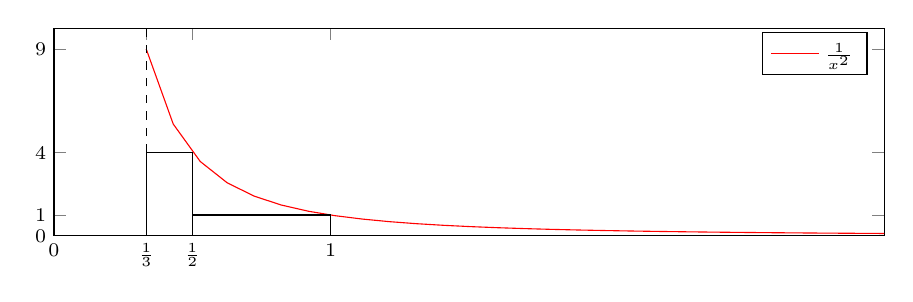
\begin{tikzpicture}
	\begin{axis}[
		height=120pt,
		width=\textwidth,
		xtick={0,1/3,1/2,1},
		xticklabels={$0$,$\frac{1}{3}$, $\frac{1}{2}$, $1$},
		ytick={0,1,4,9},
		ymin=0,ymax=10,
		xmin=0,xmax=3,
		]
	\addplot[
		domain=1/3:10,
		samples=100,
		color=red
		]{1/x^2};
	\draw[color=black, dashed] 
		(axis cs:1/3, 0) -- (axis cs:1/3, 10);
	\draw (axis cs:1/3,0) rectangle (axis cs:1/2,4);
	\draw (axis cs:1/2,0) rectangle (axis cs:1,1);
	

	\addlegendentry{\( \frac{1}{x^2} \)};
	\end{axis}
	\end{tikzpicture}
	\end{center}
	\vspace{-5pt}

	Above is the graph of $f(x)$ compared to $\frac{1}{x}^{2}$.
	\newline For $x > 1$, we have $f(x) = 0$ and for $x\in (\frac{1}{n+1}, \frac{1}{n}]$ we have $f(x) = n^{2}$
	\newline Therefore, on $(\frac{1}{3}, \infty)$, $J = \{( \frac{1}{2}, 1], ( \frac{1}{3}, \frac{1}{2}]\}$ we have
		\[f(x) = \sum_{j = 1}^{2} c_{j} \chi_{J_{j}}(x) = 4\chi_{( \frac{1}{3}, \frac{1}{2}]} + 1\chi_{( \frac{1}{2}, 1]}\]

	Therefore, via Definition 4.3, we have that
	\[\sum_{j = 1}^{2} \lvert c_{j} \rvert \lambda(J_{j}) =\lvert 1 \rvert \lambda\left( \left( \frac{1}{2}, 1\right]\right) + \lvert 4 \rvert \lambda\left( \left( \frac{1}{3}, \frac{1}{2}\right]\right) < \infty\]
	And therefore, $f$ is integrable on $(\frac{1}{3}, \infty)$, and
	\begin{align*}
		\int_{ \frac{1}{3}}^{\infty} f &= \lambda\left( \left( \frac{1}{2}, 1\right]\right) + 4\lambda\left( \left( \frac{1}{3}, \frac{1}{2}\right]\right) \\
									   &= \left(1 - \frac{1}{2}\right) + 4\left( \frac{1}{2} - \frac{1}{3}\right) = \frac{1}{2} + \frac{4}{6} = \frac{7}{6}
	\end{align*}

	\noindent\rule{\textwidth}{0.2pt}
	\textit{Discuss the Lebesgue integrability of the function $f$ on the interval $(0, 1]$. If the function is integrable, calculate the value of $\int_{0}^{1} f$}

	Proof using Monotone Convergence Theorem: Consider $f_{n} = f \chi_{(1 /n, 1]}$. Then $f_{n}\to f$ monotonically and hence $f$ is integrable on $(0, 1]$ iff
	\[\sup_{n} \int_{0}^{1} f_{n} < \infty\]
	For each $f_{n}$ we can calculate an increasing sum:
	\begin{align*}
		\int_{0}^{1} f_{n} = \int_{1 /n}^{1} f &= \sum_{k = 1}^{n - 1} k^{2} \lambda \left(\left(\frac{1}{k+1}, \frac{1}{k}\right]\right) \\
											   &= \sum_{k = 1}^{n - 1} \frac{k^{2}}{k(k+1)} =\sum_{k = 1}^{n - 1} \frac{k}{k+1} 
	\end{align*}

	Since $\frac{k}{k + 1} \to 1$ the series $\sum_{k = 1}^{\infty} \frac{k}{k+1}$ diverges, and hence
	\[\sup_{n} \int_{0}^{1} f_{n} = \infty\]
	and therefore, $f$ is \textbf{not} integrable on $(0, 1]$
\end{xmp}




\end{multicols}
\end{document}
